% Preamble

% use the beamer document class
\documentclass[hyperref={pdfpagelabels=false}, 14pt]{beamer}
% Text in square brackets is to avoid the warning: Package hyperref Warning: Option `pdfpagelabels’ is turned off (hyperref) because \thepage is undefined. Hyperref stopped early
% See: http://texblog.net/latex-archive/presentations/beamer-warnings/

% to set up the beamer class to use another colour shade, use these lines instead of the one above
%\documentclass[xcolor=dvipsnames]{beamer} 
%\usecolortheme[named=Brown]{structure}

% use Latin Modern fonts
% This also avoids the warnings: LaTeX Font Warning: Font shape `OT1/cmss/m/n’ in size <4> not available (Font) size <5> substituted on input line 6. and: LaTeX Font Warning: Size substitutions with differences  (Font) up to 1.0pt have occurred.
\usepackage{lmodern}
\usepackage{color}

\usepackage{iwona}  % cool-looking font

%\usepackage[T1]{fontenc}
%\usepackage[T1]{tipa}
%\usepackage[tipa]{ucs}
\usepackage[utf8x]{inputenc}  % required to allow accented characters like â to appear properly
\usepackage{textcomp}  % to allow arrows
\usepackage{fancyvrb}  % to allow tabs in verbatim text
\usepackage{upquote}  % ensures that an apostrophe in a verbatim environment is upright like the ASCII apostrophe

\usepackage[font=scriptsize,labelformat=empty,center,singlelinecheck=false]{caption}

\usepackage[absolute,overlay]{textpos} 
\newenvironment{reference}[2]{% 
  \begin{textblock*}{\textwidth}(#1,#2) 
      \footnotesize\it\bgroup\color{ESRCred}}{\egroup\end{textblock*}}
% provides a new reference environment for giving citations on a slide - like footnotes, except they are spread out across the slide, and not stacked; call immediately after the frametitle, with two figures giving the location on the slide:
% \begin{reference}{8mm}{80mm} ... \end{reference}
% http://www.math.umbc.edu/~rouben/beamer/quickstart-Z-H-17.html#node_sec_17

\definecolor{ESRCblue}{RGB}{47,70,148}  % ESRC blue
\definecolor{ESRCred}{RGB}{154,0,10}  % ESRC red

% replace the theme lines below with the following line to get rid of most of the colours for handouts
%\usetheme{default}

\usetheme{Boadilla}
% comment out the following line to get a white background and black text on the slide body
%\usecolortheme{albatross}

%\beamertemplateshadingbackground{blue!70}{blue!100}  % gradient full-blue to partial-blue

\setbeamercolor{structure}{fg=ESRCblue}
\setbeamerfont{frametitle}{series=\bfseries}

%\setbeamercolor{normal text}{fg=blue!30}
\setbeamertemplate{background canvas}{
\includegraphics[width=\paperwidth,height=\paperheight]{images/mainpage.jpg}}
%\setbeamertemplate{footline}{\insertframenumber/ \inserttotalframenumber}
\beamertemplatenavigationsymbolsempty  % hide navigation buttons

% specify the details to appear on the title page
\title[Bangor Autoglosser]{\newline\newline\newline \textbf{The Bangor Autoglosser:} \\ \textbf{A Multilingual Tagger for Conversational Text}}
\author[Donnelly, Deuchar]{\textbf{Kevin Donnelly, Margaret Deuchar}}
\institute[Bangor University]{\begin{normalsize} \textcolor{ESRCred}{ESRC Centre for Research on Bilingualism \\ Bangor, Wales} \end{normalsize}}
\date{}

\begin{document}

% build title page
{ % brace to limit the scope of \setbeamertemplate
\setbeamertemplate{footline}{}  % remove the footer from the title slide; using {footline}[page number]{} includes the page number
\beamertemplatenavigationsymbolsempty  % hide navigation buttons 
\setbeamertemplate{background canvas}{
\includegraphics[width=\paperwidth,height=\paperheight]{images/titlepage.jpg}}
\maketitle
} % closing brace

%============================

% The first POS-tagger for Welsh -- capable of tagging conversational speech in multiple languages.
% Multilingual discourse is far more common than has been assumed in classical linguistics


\begin{frame}
\frametitle{\begin{small}\insertframenumber/\inserttotalframenumber\end{small} The Centre}
\begin{itemize}
\item ESRC Centre for Research in Bilingualism
\item Established January 2007
% First research centre in the UK to focus specifically on bilingualism
\item Five research themes
% Neuroscience, experimental research, ethnography, speech
\item Corpus-based research
\item \textbf{bilingualism.bangor.ac.uk}
\end{itemize}
\end{frame}


\begin{frame}{Bangor corpora}
\begin{center}
\begin{tabular}{ccccc}
& \begin{small}\textit{Chats}\end{small} & \begin{small}\textit{Hours}\end{small} & \begin{small}\textit{Words}\end{small} & \begin{small}\textit{Date}\end{small} \\
\cline{1-5}\noalign{\smallskip}
\textbf{Welsh-English} & 69 & 40 & 456k & 2009 \\
(Siarad) & & & \\
\textbf{Spanish-English} & 32 & 20 & 161k & 2011 \\
(Miami) & & & \\
\textbf{Welsh-Spanish} & 31 & 20 & 126k & 2011 \\
(Patagonia) & & & \\
\hline\noalign{\smallskip}
& \textbf{132} & \textbf{80} & \textbf{743k} \\
\multicolumn{5}{l}{} \\
\multicolumn{5}{l}{All available under the GPL.}
\end{tabular}
\end{center}
\end{frame}


\begin{frame}{A sample utterance}
\begin{footnotesize}
\textbf{*SER:}   dw@1 i@1 (y)n@1 tynnu@1 llun@1 i@1 [/] i@1 (y)r@1 plant@1 $<$i@1 plant@1$>$ [//] $<$i@1 (y)r@1$>$ [//] \# i@1 er@0 \&h Helen@0 a@1 Susanna@0 a@1 +/. \%snd:"deuchar1"\_73881\_79477 \\
\bigskip
\textcolor{ESRCred}{\textbf{\%gls:} be.1S.PRES PRON.1S PRT take.NONFIN picture for for DET children for children for DET for IM Helen and Susanna and} \\
\bigskip
\textbf{\%eng:}   I draw a picture for \dots for the children, for, er, Helen and Susanna and \dots \\
\end{footnotesize}
\begin{small}
\hfill\textit{(Siarad corpus, deuchar1)} \\
\end{small}
% Hesitation markers, delivery hints, elision
\end{frame}


\begin{frame}{Transcription format \\ \begin{normalsize}CLAN: childes.psy.cmu.edu/clan \end{normalsize}}
\begin{center}
\begin{small}
\begin{tabular}{p{3cm}p{6cm}}
\multicolumn{2}{p{9cm}}{\textit{*SER dw@1 i@1 (y)n@1 hopeless@2 efo@1 tynnu@1 llun@1 . \%snd:"deuchar1"\_72848\_73881}} \\
\hline\noalign{\smallskip}
\textbf{Speaker} & *SER \\
\hline\noalign{\smallskip}
\textbf{Utterance} & \textcolor{ESRCblue}{dw@1 i@1 (y)n@1 hopeless@2 efo@1 tynnu@1 llun@1 .} \\
\hline\noalign{\smallskip}
\textbf{Language tags} & 1=Welsh, 2=English, 0=indeterminate \\
% Uses old coding 
\hline\noalign{\smallskip}
\textbf{Audio location} & \%snd:"deuchar1"\_72848\_73881 \\
\hline\noalign{\smallskip}
\textcolor{ESRCred}{\textbf{Manual gloss}} & \textcolor{ESRCred}{be.1S.PRES PRON.1S PRT hopeless with take.NONFIN picture}
% Provides lexemes and POS tags, but mainly for verbs
\end{tabular}
\end{small}
\end{center}
\end{frame}


\begin{frame}{Glossing}
\begin{itemize}
\item Allows non-native speakers to parse the conversation
\item Labour-intensive
\item Tedious
\item Inconsistent: \textit{ychydig} -- ``a\_bit''/``a\_little''
\item Tags difficult to revise later
\end{itemize}
\end{frame}


\begin{frame}{Existing options}
\begin{itemize}
\item Spanish -- CLAN $\rightarrow$ MOR + POST
\item Welsh -- no tagger at all
\end{itemize}
\end{frame}


\begin{frame}{Aims}
\begin{itemize}
\item Tag across multiple languages simultaneously
\item Single application infrastructure
\item Handle conversational language
\item Use FOSS where possible
\begin{itemize}
    \item speed of development
    \item re-use scarce language resources
    \item bootstrap new languages easily
\end{itemize}
\end{itemize}
\end{frame}


\begin{frame}{}
\begin{center}
\begin{huge} \textcolor{ESRCred}{Dictionaries} \end{huge}
\end{center}
\end{frame}


\begin{frame}{Dictionary format}
\begin{itemize}
\item Derived from GPL or PD resources
% Eurfa, Apertium, Kevin Atkinson/Grady Ward
\item One database table
\item Words, not morphemes
\item Easily presented in a spreadsheet
% May be less forbidding than a database to most linguists
\item Easy to update
\item Easy to get started
% Any basic wordlist will do
\end{itemize}
\end{frame}


\begin{frame}{Welsh dictionary}
\begin{center}
\begin{small}
\begin{tabular}{ccccccc}
\textit{surface} & \textit{lemma} & \textit{enlemma} & \textit{pos} & \textit{gender} & \textit{number} & \textit{tense} \\
\hline\noalign{\smallskip}
\textbf{bara} & bara & bread & n & m & sg & \\
\hline\noalign{\smallskip}
\textbf{cathod} & cath & cat & n & f & pl & \\
\hline\noalign{\smallskip}
\textbf{mynd} & mynd & go & v & & & infin \\
\hline\noalign{\smallskip}
\textbf{aeth} & mynd & go & v & & 3s & past \\
\hline\noalign{\smallskip}
\textbf{hapus} & hapus & happy & adj & &  & \\
\hline\noalign{\smallskip}
\textbf{rhywsut} & rhywsut & somehow & adv & & & \\
\hline\noalign{\smallskip}
\textbf{heb} & heb & without & prep & & & \\
\hline\noalign{\smallskip}
\end{tabular}
% Quite simple
% Easily accessible to non-CS people
\end{small}
\end{center}
\end{frame}


\begin{frame}{Spanish dictionary}
\begin{center}
\begin{small}
\begin{tabular}{ccccccc}
\textit{surface} & \textit{lemma} & \textit{enlemma} & \textit{pos} & \textit{gender} & \textit{number} & \textit{tense} \\
\hline\noalign{\smallskip}
\textbf{perro} & perro & dog & n & m & sg & \\
\hline\noalign{\smallskip}
\textbf{canciones} & canción & song & n & f & pl & \\
\hline\noalign{\smallskip}
\textbf{empezar} & empezar & start & v & & & infin \\
\hline\noalign{\smallskip}
\textbf{empieza} & empezar & start & v & & 23s & pres \\
\hline\noalign{\smallskip}
\textbf{empieza} & empezar & start & v & & 2s & imper \\
\hline\noalign{\smallskip}
\textbf{rojo} & rojo & red & adj & m & sg & \\
\hline\noalign{\smallskip}
\textbf{rojas} & rojo & red & adj & f & pl & \\
\hline\noalign{\smallskip}
\textbf{por} & por & for & prep & & & \\
\hline\noalign{\smallskip}
\end{tabular}
% Quite simple
% Easily accessible to non-CS people
\end{small}
\end{center}
\end{frame}


\begin{frame}
\frametitle{\begin{small}\insertframenumber/\inserttotalframenumber\end{small} English dictionary}
\begin{center}
\begin{small}
\begin{tabular}{ccccccc}
\textit{surface} & \textit{lemma} & \textit{pos} & \textit{number} & \textit{tense} \\
\hline\noalign{\smallskip}
\textbf{break} & break & sv & & infin \\
\hline\noalign{\smallskip}
\textbf{broke} & break & av & & past \\
\hline\noalign{\smallskip}
\textbf{broken} & break & av & & pastpart \\
\hline\noalign{\smallskip}
\textbf{car} & car & n & sg & \\
\hline\noalign{\smallskip}
\textbf{quick} & adj & & & \\
\hline\noalign{\smallskip}
\textbf{by} & by & prep & & \\
\hline\noalign{\smallskip}
\textbf{which} & which & rel & & \\
\hline\noalign{\smallskip}
\end{tabular}
% Simpler layout - one entry for ``break'' a clean break, break the bank, they break the rules
% Gender field is available, but not really used.  Enlemma just repeats surface.
\\ \medskip
\begin{footnotesize}\textit{breaks, breaking, cars, quickly} are derived during lookup\end{footnotesize}
\end{small}
\end{center}
\end{frame}


\begin{frame}{}
\begin{center}
\begin{huge} \textcolor{ESRCred}{The autoglossing process} \end{huge}
\end{center}
\end{frame}


\begin{frame}{Stages in the \\ autoglossing process}
\begin{itemize}
\item \textbf{Stage 1 }-- Import the unglossed file
\item \textbf{Stage 2} -- Look up the words it contains
\item \textbf{Stage 3} -- Disambiguate between alternatives for a word
\item \textbf{Stage 4} -- Output the glossed file
\end{itemize}
\end{frame}


\begin{frame}{Stage 1 \\ Import the chat file}
\begin{itemize}
% Don't need to spend too much time on this
\item Read each line of the file into an utterances table
\item Select the utterance and discard non-word material
\item Split the resulting utterance into words
\item Put them into a words table
%\item Handles 4 different language-tagging systems
% Different transcribers have worked on the corpora over the 5-year period
% CLAN itself has changed its system
% Earlier sample showed 0,1,2 for language-tags
% Current one only tags non-default items with the ISO 3-letter tag
\end{itemize}
\end{frame}


\begin{frame}{Sample import}
\begin{center}
\begin{small}
\begin{tabular}{p{3cm}p{6cm}}
\multicolumn{2}{p{9cm}}{\textit{*SOF: $<$y si$>$ [/] y si entra algún camión ahí por ejemplo a dejar muebles o cualquier cosa . }} \\
\hline\noalign{\smallskip}
\textbf{Speaker} & *SOF \\
\hline\noalign{\smallskip}
\textbf{Utterance} & \textcolor{ESRCblue}{y si entra algún camión ahí por ejemplo a dejar muebles o cualquier cosa .}\\
\hline\noalign{\smallskip}
\textbf{English} & And if some lorry goes in there, for example, to leave off furniture or whatever.
\end{tabular}
\vskip 0.5cm
\hfill\textit{(Miami corpus, sastre1)}
\end{small}
\end{center}
\end{frame}


\begin{frame}{The words table}
  \begin{figure}[h]
  \centering
  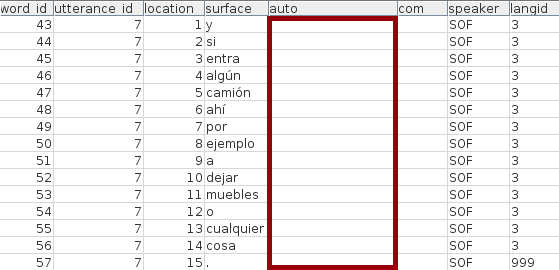
\includegraphics[width=\textwidth]{images/words_table1.png}
  \end{figure}
  % Spanish sentence from the Miami corpus.
  % At this stage the autogloss field would be empty - that is what we're going to add now.
\end{frame}


\begin{frame}{Stage2 \\ Dictionary lookup}
\begin{itemize}
\item Using the language tag, look up each word against the appropriate dictionary
\item Do basic segmentation (e.g clitic pronouns in Spanish, verb-tenses in English, mutation in Welsh)
\item Write out all the dictionary entries (readings) for that word
\item Feed these to the constraint grammar parser for disambiguation
\end{itemize}
\end{frame}


\begin{frame}{Constraint Grammar}
\begin{itemize}
\item Developed by Fred Karlsson in the 90s
\item Third generation of the parser: \textbf{visl-cg3}
\item Eckhard Bick, Tino Didriksen
\item Free (GPL) license
\item \textbf{beta.visl.sdu.dk/constraint\_grammar.html}
\item Easily-understood rules
\end{itemize}
\end{frame}


\begin{frame}{Stage 3 \\ Disambiguation}
\begin{itemize}
\item \begin{large}\textbf{select (n) if (-1 (ord));} \end{large}
\item Choose the noun (\textbf{n}) reading if the first word to the left (\textbf{-1}) is an ordinal (\textbf{ord})
\item Welsh: \textit{yr ail dro} (the second time)
\item English: \textit{the third man}
\item Spanish: \textit{el primer viaje} (the first journey)
\item Verb readings for \textit{dro}, \textit{man} and \textit{viaje} will be deleted
% 
\end{itemize}
\end{frame}


\begin{frame}{Language-specific rules}
\begin{itemize}
\item Include that language's tag in the rule to constrain its application
\item \begin{large}\textbf{select ([es] n) if (-1 ([es] ord));} \end{large}
\item Now applies only to Spanish: \textit{el primer viaje}
% 
\end{itemize}
\end{frame}


\begin{frame}[fragile]{Before disambiguation}
\begin{footnotesize}
\begin{BVerbatim}
"<ddim>"
    "dim"  {96,1} [cy] n m sg :nothing: [208789] + sm
    "dim"  {96,1} [cy] adv :not: [204176] + sm
"<yn>"
    "yn"  {96,2} [cy] stat :stative: [200654]
    "yn"  {96,2} [cy] prep :in: [204430]
    "gan"  {96,2} [cy] prep :with: [196964] + sm
"<gynnar>"
    "cynnar"  {96,3} [cy] adj :early: [209212] + sm
"<iawn>"
    "iawn"  {96,4} [cy] adv :OK: [207540]
    "iawn"  {96,4} [cy] adv :very: [203775]
\end{BVerbatim}
\\ \hfill\textit{(Patagonia corpus, patagonia1)}
\end{footnotesize}
\\ ``\textit{not very early}''
\end{frame}


\begin{frame}[fragile]{After disambiguation}
\begin{footnotesize}
\begin{BVerbatim}
"<ddim>"
    "dim" {96,1} [cy] adv :not: [204176] + sm
"<yn>"
    "yn" {96,2} [cy] stat :stative: [200654]
"<gynnar>"
    "cynnar" {96,3} [cy] adj :early: [209212] + sm
"<iawn>"
    "iawn" {96,4} [cy] adv :very: [203775]
\end{BVerbatim}
\\ \hfill\textit{(Patagonia corpus, patagonia1)}
\end{footnotesize}
\\ ``\textit{not very early}''
\end{frame}


\begin{frame}{Stage 4 \\ Output the glossed file}
\begin{itemize}
\item Read the disambiguated constraint grammar output
\item Insert each lexeme and its part-of-speech tags into the words table
\item Use the utterances and words tables to write out an autoglossed file
% 
\end{itemize}
\end{frame}


\begin{frame}{The words table}
  \begin{figure}[h]
  \centering
  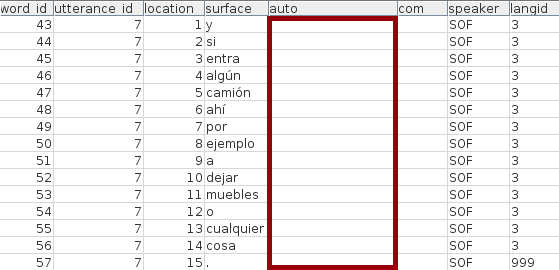
\includegraphics[width=\textwidth]{images/words_table1.png}
  \end{figure}
  % Spanish sentence from the Miami corpus.
  % At this stage the autogloss field would be empty - that is what we're going to add now.
\end{frame}


\begin{frame}{The words table -- glossed}
  \begin{figure}[h]
  \centering
  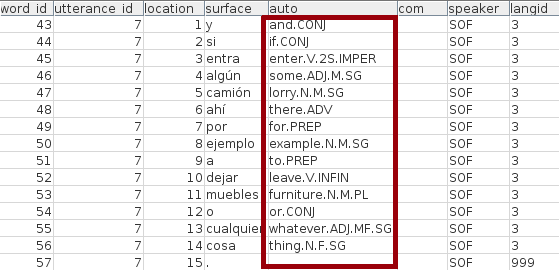
\includegraphics[width=\textwidth]{images/words_table.png}
  \end{figure}
  % Spanish sentence from the Miami corpus.
  % The autogloss field is now filled.
\end{frame}


\section{Evaluation}


\begin{frame}{}
\begin{center}
\begin{huge} \textcolor{ESRCred}{Evaluation} \end{huge}
\end{center}
\end{frame}


\begin{frame}{Speed}
\begin{itemize}
\item 900-1100 words per minute
\item 1 minute to autogloss 5 minutes of speech
\item Siarad: 500,000 words in 8h27m
% 
\end{itemize}
\end{frame}


\begin{frame}{Accuracy}
\begin{center}
\begin{tabular}{ccccc}
& \begin{small}\textit{Words}\end{small} & \begin{small}\textit{Coverage}\end{small} & \begin{small}\textit{MFL}\end{small} & \begin{small}\textit{Accuracy}\end{small} \\
\cline{1-5}\noalign{\smallskip}
\textbf{Welsh-Spanish} & 15,677 & 100\% & W:92\% & 99\% \\
(Patagonia\footnote{patagonia1,2,3,6}) & & & S:1\% \\
\textbf{Welsh-English} & 10,411 & 96\% & W:81\% & 98\% \\
(Siarad\footnote{deuchar1, stammers4}) & & & E:2\% \\
\textbf{Spanish-English} & 10,411 & 97\% & E:54\% & 96\% \\
(Miami\footnote{herring7, sastre1, zeledon5}) & & & S:42\% \\
\end{tabular}
\end{center}
\end{frame}


\begin{frame}{Comparison with \\ other methods}
\begin{itemize}
\item Spanish -- MOR glosser (part of the CLAN suite)
\item Welsh -- manual (human) glossing
\item Two sample files from each corpus glossed using both methods
\item Aligned and then inspected manually
\item Typos or missing lexemes not counted as errors
\item Names omitted from consideration
\end{itemize}
\end{frame}


\begin{frame}{Comparison between \\ autoglosser and MOR}
  \begin{figure}[h]
  \centering
  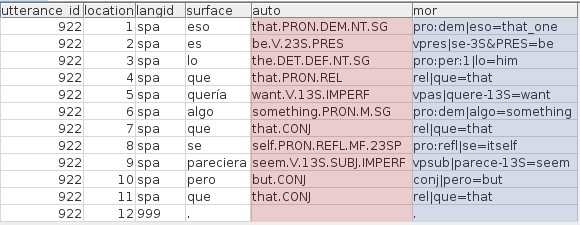
\includegraphics[width=\textwidth]{images/comp.png}
  \end{figure}
  %
\end{frame}


\begin{frame}{Spanish files}
\begin{itemize}
\item Tested on \textit{herring11}, \textit{sastre5}
\item 8,039 tokens, 1,638 types (TTR: 0.20)
\end{itemize}
\begin{center}
\begin{tabular}{cc}
\multicolumn{2}{c}{\textit{Language mix}} \\
\cline{1-2}\noalign{\smallskip}
\textbf{Spanish}     & 88\% \\
\textbf{English}    & 9\% \\
\textbf{indeterminate}    & 3\% \\
\end{tabular}
\end{center}
\end{frame}


\begin{frame}{Welsh files}
\begin{itemize}
\item Tested on \textit{stammers7}, \textit{stammers9}
\item 9,454 tokens, 1,376 types (TTR: 0.15)
\end{itemize}
\begin{center}
\begin{tabular}{cc}
\multicolumn{2}{c}{\textit{Language mix}} \\
\cline{1-2}\noalign{\smallskip}
\textbf{Welsh}     & 87\% \\
\textbf{English}    & 2\% \\
\textbf{indeterminate}    & 11\% \\
\end{tabular}
\end{center}
\end{frame}


\begin{frame}{Comparison with MOR  \\ glossing (Spanish)}
\begin{reference}{17mm}{80mm}  % a slide is 128mm×96mm; 8mm in and 80mm down from top left
    * wrong lexeme 0.7\%, wrong POS 0.2\%, ambiguous 1.7\%\\
    $^\dag$ wrong lexeme 1.6\%, wrong POS 0.7\%, ambiguous 0.1\%\\
\end{reference}
\begin{Large}
\begin{center}
\begin{tabular}{ccc}
& \textit{Autoglosser} & \textit{MOR} \\ 
\cline{1-3}\noalign{\smallskip}
\textbf{Coverage}     & \textcolor{ESRCred}{96.9\%} & \textcolor{ESRCblue}{95.7\%} \\
\textbf{Accuracy}    & \textcolor{ESRCred}{97.4\%*} & \textcolor{ESRCblue}{97.6\%$^\dag$} \\
\end{tabular}
\end{center}
\end{Large}
\end{frame}


\begin{frame}{Comparison with manual \\ glossing (Welsh)}
\begin{reference}{15mm}{80mm}  % a slide is 128mm×96mm; 8mm in and 80mm down from top left
    * wrong lexeme 0.7\%, wrong POS 0.1\%, ambiguous 1.4\%\\
\end{reference}
\begin{Large}
\begin{center}
\begin{tabular}{ccc}
& \textit{Autoglosser} & \textit{Human} \\ 
\cline{1-3}\noalign{\smallskip}
\textbf{Coverage}     & \textcolor{ESRCred}{98.3\%} & \textcolor{ESRCblue}{99.9\%} \\
\textbf{Accuracy}    & \textcolor{ESRCred}{97.9\%*} & \textcolor{ESRCblue}{99.9\%} \\
\end{tabular}
\end{center}
\end{Large}
\end{frame}


\section{Spin-off benefits}


\begin{frame}{}
\begin{center}
\begin{huge} \textcolor{ESRCred}{Spin-off benefits} \end{huge}
\end{center}
\end{frame}


\begin{frame}{Typesetting -- before}
\begin{footnotesize}

\textbf{*SER:}   dw@1 i@1 (y)n@1 hopeless@2 efo@1 tynnu@1 llun@1 . \%snd:"deuchar1"\_72848\_73881

\textit{\%gls:}   be.1S.PRES PRON.1S PRT hopeless with take.NONFIN picture

\textit{\%eng:}   I'm hopeless at drawing

\textbf{*SER:}   dw@1 i@1 (y)n@1 tynnu@1 llun@1 i@1 [/] i@1 (y)r@1 plant@1 $<$i@1 plant@1$>$ [//] $<$i@1 (y)r@1$>$ [//] \# i@1 er@0 \&h Helen@0 a@1 Susanna@0 a@1 +/. \%snd:"deuchar1"\_73881\_79477

\textit{\%gls:}   be.1S.PRES PRON.1S PRT take.NONFIN picture for for DET children for children for DET for IM Helen and Susanna and

\textit{\%eng:}   I draw a picture for \dots for the children, for, er, Helen and Susanna and \dots

\end{footnotesize}
\begin{small}
\hfill\textit{(Siarad corpus, deuchar1)}
\end{small}
% Hesitation markers, delivery hints, elision
\end{frame}


\begin{frame}{Typesetting -- after}
  \begin{figure}[h]
  \centering
  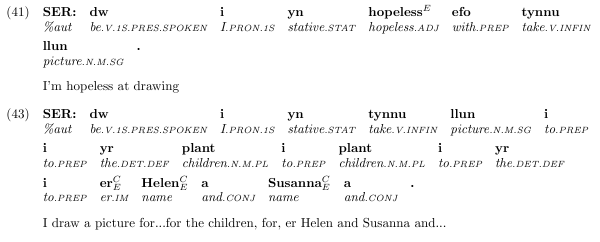
\includegraphics[scale=0.7]{images/deuchar1.png}
  \end{figure}
\end{frame}


\begin{frame}{Conversation profile \\ \begin{normalsize}Spanish-English\end{normalsize}}
  \begin{figure}[h]
  \centering
  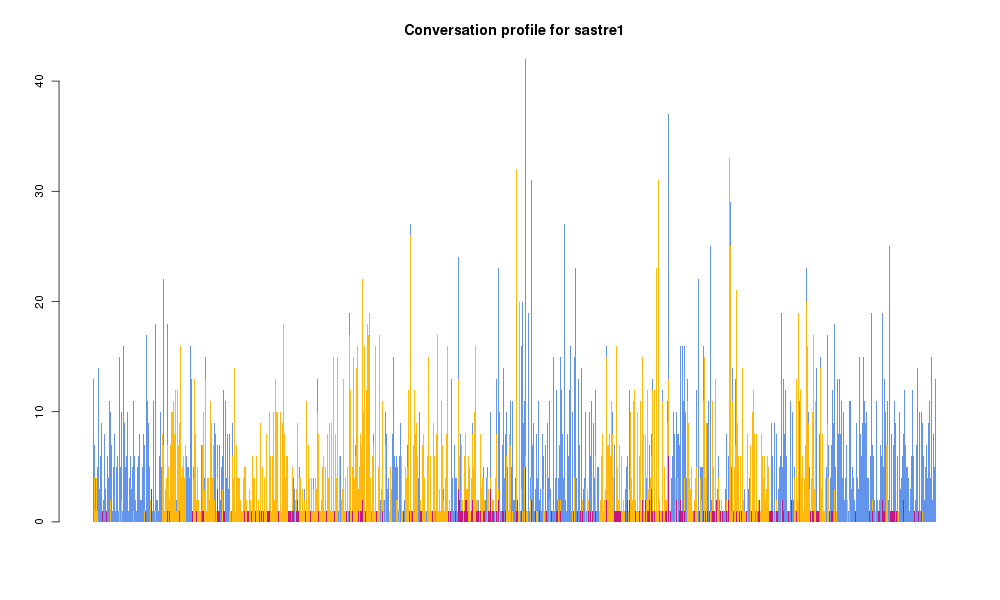
\includegraphics[scale=0.3]{images/allsastre1.png}
  \end{figure}
\end{frame}


\begin{frame}{Conversation profile \\ \begin{normalsize}Welsh-English\end{normalsize}}
  \begin{figure}[h]
  \centering
  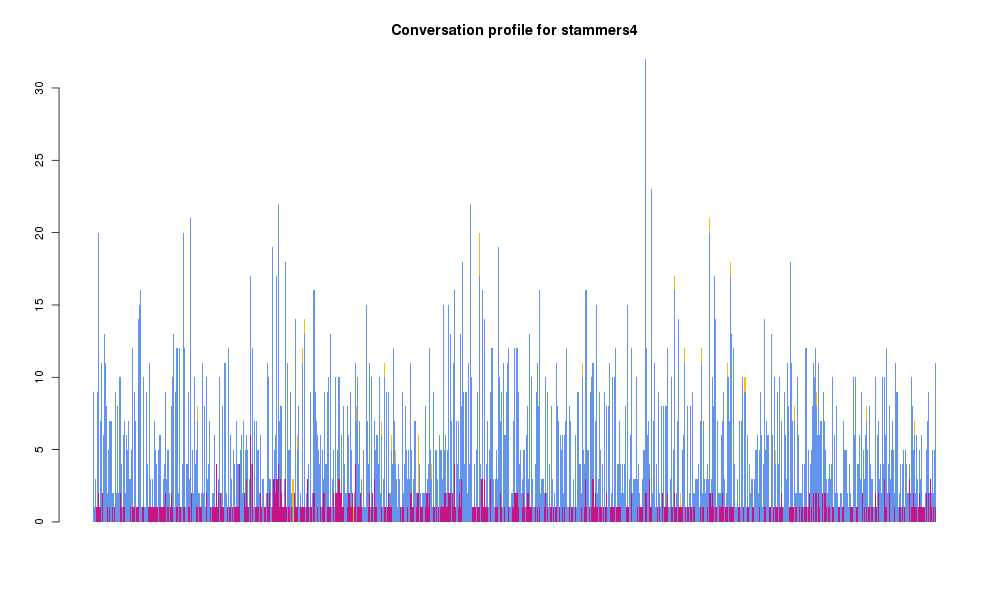
\includegraphics[scale=0.3]{images/allstammers4.png}
  \end{figure}
\end{frame}


\begin{frame}{Mixed Collocations \\ \begin{normalsize}Det+Noun+Adj\end{normalsize}}
\begin{itemize}
\item un healthy store (\textit{a healthfood store})
\item the mismo papel (\textit{the same paper})
\item the fair estúpido (\textit{the stupid fair})
\item la cheerleader pesada (\textit{the plump cheerleader})
\item un dealer grande (\textit{a big dealer})
\item un pequeño pocket (\textit{a little pocket})
\end{itemize}
\textbf{26} trigrams out of \textbf{161,000} words \dots \\
\hfill \dots difficult to find manually
\end{frame}


\begin{frame}{}
\begin{center}
\begin{huge} \textcolor{ESRCred}{Resources} \end{huge}
\end{center}
\end{frame}


\begin{frame}{}
\begin{center}
\begin{LARGE} \textcolor{ESRCred}{bangortalk.org.uk} \end{LARGE} \\
\bigskip
Web-interface to the transcripts \\
\bigskip
Transcript and audiofile download \\
\bigskip
Bangor Autoglosser code (Git repository) \\
Licensed under GPL v3
\end{center}
\end{frame}


\end{document}